%# -*- coding: utf-8-unix -*-
%======================================================================
% qbook.tex for Qbook Template
%======================================================================
% 双面打印
\documentclass{qbook}

\addbibresource{bib/qbook.bib}  % 导入参考文献数据库
\begin{document}
\pagestyle{empty}
%# -*- coding: utf-8-unix -*-
\thispagestyle{empty}
\begin{tikzpicture}[overlay,remember picture,font=\sffamily\bfseries]
\draw[ultra thick,c4,name path=big arc] ([xshift=-2mm]current page.north) arc(150:285:11)
coordinate[pos=0.225] (x0);
\begin{scope}
\clip ([xshift=-2mm]current page.north) arc(150:285:11) --(current page.north
east);
\fill[c4!50,opacity=0.25] ([xshift=4.55cm]x0) circle (4.55);
\fill[c4!50,opacity=0.25] ([xshift=3.4cm]x0) circle (3.4);
\fill[c4!50,opacity=0.25] ([xshift=2.25cm]x0) circle (2.25);
\draw[ultra thick,c4!50] (x0) arc(-90:30:6.5);
\draw[ultra thick,c4] (x0) arc(90:-30:8.75);
\draw[ultra thick,c4!50,name path=arc1] (x0) arc(90:-90:4.675);
\draw[ultra thick,c4!50] (x0) arc(90:-90:2.875);
\path[name intersections={of=big arc and arc1,by=x1}];
\draw[ultra thick,c4,name path=arc2] (x1) arc(135:-20:4.75);
\draw[ultra thick,c4!50] (x1) arc(135:-20:8.75);
\path[name intersections={of=big arc and arc2,by={aux,x2}}];
\draw[ultra thick,c4!50] (x2) arc(180:50:2.25);
\end{scope} 
\path[decoration={text along path,text color=c4,
	raise = -2.8ex,
	text  along path,
	text = {|\sffamily\bfseries|\today},
	text align = center,
},
decorate
] ([xshift=-2mm]current page.north) arc(150:245:11);
%
\begin{scope}
\path[clip,postaction={fill=c3}]
([xshift=2cm,yshift=-8cm]current page.center) rectangle ++ (4.2,7.7);
\fill[c2] ([xshift=0.5cm,yshift=-8cm]current page.center)
([xshift=0.5cm,yshift=-8cm]current page.center)  arc(180:60:2)
|- ++ (-3,6) --cycle;
\draw[ultra thick,c4] ([xshift=-1.5cm,yshift=-8cm]current page.center) 
arc(180:0:2);
\draw[ultra thick,c4] ([xshift=0.5cm,yshift=-8cm]current page.center) 
arc(180:0:2);
\draw[ultra thick,c4] ([xshift=2.5cm,yshift=-8cm]current page.center) 
arc(180:0:2);
\draw[ultra thick,c4] ([xshift=4.5cm,yshift=-8cm]current page.center) 
arc(180:0:2);
\fill[red] ([xshift=2.5cm,yshift=-8cm]current page.center) +(60:2) circle(1.5mm);
\node[text=c5!80!black] at ([xshift=4.7cm,yshift=-5.2cm]current page.center) {$\rho:=\dfrac{1+\sqrt{-3}}{2}$};
\end{scope}
%
\fill[c1] ([xshift=2cm,yshift=-8cm]current page.center) rectangle ++ (-13.7,7.7);
\node[text=white,anchor=west,scale=4,inner sep=0pt] at
([xshift=-8cm,yshift=-3cm]current page.center) {微~分~几~何};
\node[text=white,anchor=west,scale=2,inner sep=0pt] at
([xshift=-3.3cm,yshift=-5.5cm]current page.center) {333~制作};
\end{tikzpicture}  % 载入封面
\newpage
\begin{center}
	\Large{\sffamily\bfseries\heiti Version 2.02} \\ \vspace{2em}
	\Large{\sffamily\bfseries\heiti 编译日期: \today} \\ \vspace{1em}
	\Large{\sffamily\bfseries\heiti 任何建议及错误信息请发送至邮箱} \\
	\texttt{jey74165@163.com}
\end{center} 
\vfill
\vspace{30em}
\begin{tabular*}{\textwidth}{ccc}
	\includegraphics{figure/by-nc.eps}
	& \begin{minipage}[b]{0.6\textwidth}
		\small\sffamily
		本作品采用知识共享 署名-非商业性使用 4.0 国际 许可协议进行许可. 访问\url{http://creativecommons.org/licenses/by-nc/4.0/  }查看该许可协议.
	\end{minipage}
\end{tabular*}  
\thispagestyle{empty}
\frontmatter  % 对前言和概览用罗马数字作为页码
\pagestyle{empty}

\begin{pre}
	\thispagestyle{empty}
	\begin{center}
		{\kaishu{人在春风和气中,书到用时方恨少}}
	\end{center}

\vspace*{5\baselineskip}
\centerline{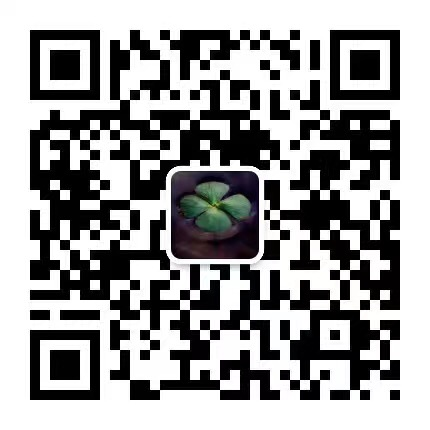
\includegraphics[scale=0.6]{example/gzh.jpg}}
\centerline{\fontsize{26pt}{26pt} 微信公众号}
\end{pre}
\pagestyle{empty}
\tableofcontents
\cleardoublepage
%# -*- coding: utf-8-unix -*-
\begin{overview}
\thispagestyle{empty}
在2018年3月底,翻译\footnote{这个模板原本是用于一项书籍翻译计划的,关注我公众号的读者对此有所了解。然而由于版权原因,该译本无法公开分享。}进度已过大半,于是开始着手进行\LaTeX 排版。在此之前我对\LaTeX 的了解微乎其微,甚至第一次安装TexLive就出了问题,不得不重新安装。也是借着给这个译本排版的机会,才逐渐熟悉了这一软件的使用方法。

如大家所见,模板的封面和扉页设计均高仿\footnote{李老师的书籍源码尚未公开,此为仿作。}自李文威老师《模形式初步》一书,并已得到李老师的使用许可;定理和定义环境则取材自网上流传的Elegantbook模版。我也从这一以模仿为主的学习过程中,对\LaTeX 有了更深入的了解。

本模板命名为$\mathbb{ Q }$-book,谐音自cubic一词。由于是一个菜鸟的作品,自然还有许多瑕疵,对此模板的错误和不足之处还请各位多多包涵。

\end{overview}
 
\mainmatter	  % 对正文用阿拉伯数字作为页码
%======================================================================
% 正文内容
\pagestyle{fancy}
\setcounter{page}{0}
\setcounter{chapter}{-1}
%# -*- coding: utf-8-unix -*-
%%==================================================
\chapter{ 预备知识}
\section{赋范向量空间} 

\begin{mydef}{范数}{1}
	内容...
\end{mydef}

根据\rdef{def:1}可知,balalala


\subsection{有界线性算子}

\begin{mythm}{闭图像定理}{2}
	内容...
\end{mythm}

根据\rthm{thm:2}可知,balalala

\begin{myprop}{}{3}
	有限维赋范空间上的范数全部等价.
\end{myprop}

根据\rprop{prop:3}可知,balalala


\begin{mylem}{Riesz引理}{4}
	内容...
\end{mylem}

根据\rlem{lem:4}可知,balalala

\begin{example}[$L^{p}(\Omega)$]
	\label{exa:1}
	内容...
\end{example}

根据\ref{exa:1}可知,。。。

\begin{proof}
	内容...
\end{proof}

%# -*- coding: utf-8-unix -*-
%%==================================================




%# -*- coding: utf-8-unix -*-


%# -*- coding: utf-8-unix -*-
%%==================================================

\include{tex/chapter5}
\include{tex/chapter6}
\include{tex/chapter7}



\include{tex/chapter9}
\include{tex/chapter10}
\backmatter	
%======================================================================
% 打印参考文献
\printbibliography[heading=bibintoc]
\makeatletter
\makeatother
\end{document}